\documentclass[%
substylefile = laboratory.rtx, % тип документа
natbib,         % использовать пакет natbib для "сжатия" цитирований
subf,           % использовать пакет subcaption для вложенной нумерации рисунков
href,           % использовать пакет hyperref для создания гиперссылок
colorlinks=true % цветные гиперссылки
%,fixint=false  % отключить прямые знаки интегралов
,times          % шрифт Times как основной
%,mtpro         % шрифт Times для формул
]{gost732-b}


\usepackage[
  a4paper, mag=1000,
  left=3.0cm, right=1cm, top=2cm, bottom=2.0cm, headsep=0.7cm, footskip=1cm
]{geometry}
\usepackage[X2, T2A]{fontenc}
\usepackage[utf8x]{inputenc}
\usepackage[english,russian]{babel}
% Многостраничные таблицы
\usepackage{tabularx,longtable,tabu,multirow}
\ifpdf\usepackage{epstopdf}\fi

% Настройка таблиц
\newcolumntype{C}{>{\centering\arraybackslash}X }

% Альбомная ориентация страниц
\usepackage{lscape}

% Плавающие рисунки "в оборку".
\usepackage{wrapfig}

% Пакет для вывода текста в несколько колонок
\usepackage{multicol}

% Пакет для листингов прогармм
\usepackage{minted}
\setminted{numbers=left, fontsize=\small, breaklines, autogobble, baselinestretch=1.1, tabsize=4, outencoding=utf8}

% Пакет для изменения межстрочного интервала
%\usepackage{setspace}

% Нумерация списков цифрами, потом буквами
% \renewcommand\theenumi  {\arabic{enumi}}
% \renewcommand\theenumii {\asbuk{enumii}}

% Номера страниц сверху и справа
\pagestyle{headright}
\chapterpagestyle{headright}

% Точка с запятой в качестве разделителя между номерами цитирований
%\setcitestyle{semicolon}

% Использовать полужирное начертание для векторов
%\let\vec=\mathbf

% Включать подсекции в оглавление
\setcounter{tocdepth}{2}

\graphicspath{{fig/}}

% Библитека для рисования фигур
\usepackage{tikz}

\begin{document}

\clubpenalty=10000 
\widowpenalty=10000

% Переопределение стандартных заголовков
%\def\contentsname{Содержание}
\def\conclusionname{Выводы}
%\def\bibname{Литература}

\institution{Государственное образовательное учреждение\\
высшего профессионального образования\\
<<Донецкий национальный технический университет>>}

% Кафедра
\chair{Кафедра программной инженерии}

% Факультет
\department{Факультет компьютерных наук и технологий}

% Имя лица, допускающего к защите (зав. кафедрой)
\apname{Федяев~О.~И.}

\title{Отчет}

\subtitle{по лабораторной работе №~1\\ по курсу <<Системы искусственного интеллекта>>}

\topic{Инженерия извлечения знаний при создании базы знаний интеллектуальной системы}

\keywords{Ключевые слова}

% Автор
\author{Воробьёв~Л.~О.} % ФИО
\group{ИПО-14б} % Группа
\coursenum{6.050103} % Номер специальности
\course{Программная инженерия} % Название специальности

% Научный руководитель
\sa      {Федяев~О.~И.}
\sastatus{доц.~каф.~ПИ}

% Город и год
\city{Донецк}
\date{\number\year}

\maketitle

%%
%% Titlepage in English
%%
%
%\institution{Doneck national texnecial university}
%
%% Approved by
%\apname{Docent A.\,I.~Andruxin}
%
%\title{Bachelor's Thesis}
%
%% Topic
%\topic{Develop SMDB for automatize manade autoschools}
%
%% Author
%\author{Author's Name} % Full Name
%\course{Program ingeenering} % Название специальности
%
%\group{} % Study Group
%
%% Scientific Advisor
%\sa       {I.\,I.~Ivanov}
%\sastatus {Professor}
%
%% Reviewer
%\rev      {P.\,P.~Petrov}
%\revstatus{Associate Professor}
%
%% City & Year
%\city{Saint Petersburg}
%\date{\number\year}
%
%\maketitle[en]

% Содержание
% \tableofcontents

% Глава 1
\chapter{Ход работы}

\section{Задание на лабораторную работу}

Разработать продукционную экспертную систему на Прологе для решения
задачи по определению группы дорожного знака.

\section{Диаграммы}

\begin{figure}[H]
	\centering
	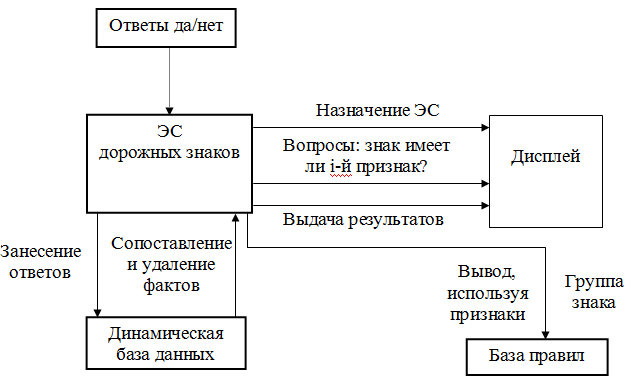
\includegraphics[width=1\linewidth]{fig/dataflow}
	\caption{Диаграмма потоков данных ЭС}
	\label{fig:dataflow}
\end{figure}

\begin{figure}[H]
	\centering
	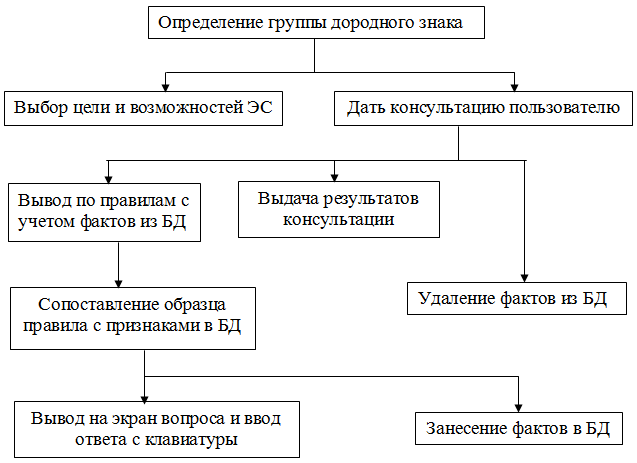
\includegraphics[width=1\linewidth]{fig/scheme}
	\caption{Структурная схема ЭС}
	\label{fig:scheme}
\end{figure}

\section{Программа на языке Prolog}

\inputminted[encoding=cp866]{prolog}{src/Prog.pro}

\begin{figure}[H]
	\centering
	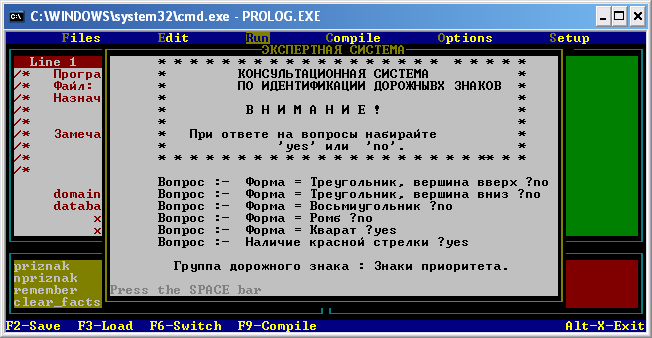
\includegraphics{fig/screen1}
	\caption{Тестирование продукционного правила 6}
	\label{fig:screen1}
\end{figure}

\begin{figure}[H]
	\centering
	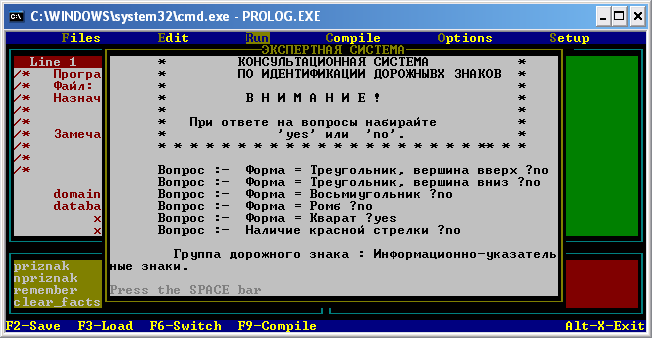
\includegraphics{fig/screen2}
	\caption{Тестирование продукционного правила 5}
	\label{fig:screen2}
\end{figure}

\begin{figure}[H]
	\centering
	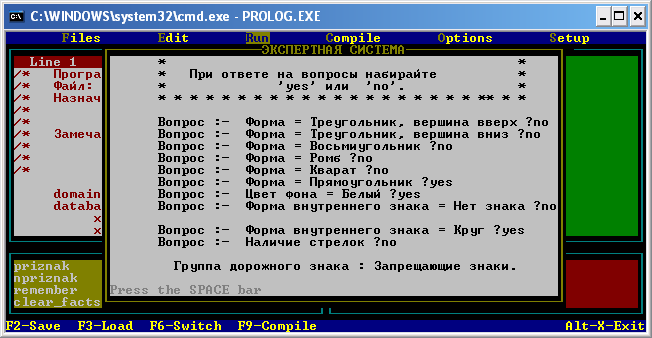
\includegraphics{fig/screen3}
	\caption{Тестирование продукционного правила 15}
	\label{fig:screen3}
\end{figure}

\begin{figure}[H]
	\centering
	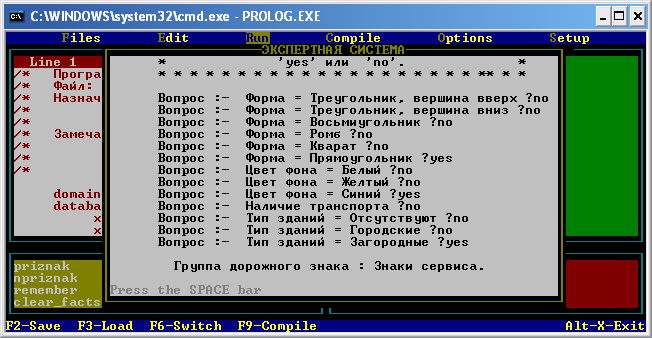
\includegraphics{fig/screen4}
	\caption{Тестирование продукционного правила 21}
	\label{fig:screen4}
\end{figure}

% Глава 2
% \section{Процесс получения дерева решений из таблицы}

Анализируется таблица от 1 до 40.
$$ 
\begin{array}{l|c|ccccccccc}
	  & C_{0} & C_{1} & C_{2} & C_{3} & C_{4} & C_{5} & C_{6} & C_{7} & C_{8} & C_{9}\\
 \textrm{GAIN} & 1.56 & 1.31 & 0.79 & 0.40 & 0.42 & 0.65 & 0.21 & 0.81 & 0.51 & 0.26
\end{array}
 $$

$$
T = \left| \begin{array}{lc|c|ccccccccc}
	 & G & C_{0} & C_{1} & C_{2} & C_{3} & C_{4} & C_{5} & C_{6} & C_{7} & C_{8} & C_{9}\\
	1 & 0 & 0 & 0 & 1 & 0 & 0 & 0 & 0 & 0 & 0 & 0\\
	2 & 0 & 0 & 1 & 1 & 0 & 0 & 0 & 0 & 0 & 0 & 0\\
	3 & 0 & 0 & 0 & 1 & 0 & 0 & 0 & 0 & 1 & 0 & 0\\
	4 & 0 & 0 & 0 & 1 & 0 & 0 & 0 & 0 & 0 & 1 & 0\\
	5 & 1 & 1 & 0 & 1 & 0 & 0 & 0 & 0 & 0 & 0 & 0\\
	6 & 1 & 2 & 3 & 0 & 0 & 0 & 0 & 0 & 4 & 0 & 0\\
	7 & 1 & 3 & 1 & 1 & 0 & 0 & 0 & 0 & 0 & 0 & 0\\
	8 & 4 & 4 & 2 & 0 & 0 & 0 & 0 & 0 & 1 & 0 & 0\\
	9 & 4 & 4 & 0 & 0 & 0 & 0 & 0 & 0 & 0 & 0 & 0\\
	10 & 1 & 4 & 2 & 0 & 0 & 0 & 1 & 1 & 0 & 0 & 0\\
	11 & 4 & 4 & 2 & 0 & 0 & 0 & 1 & 0 & 0 & 0 & 0\\
	12 & 0 & 5 & 0 & 0 & 0 & 0 & 0 & 0 & 0 & 0 & 0\\
	13 & 0 & 5 & 3 & 0 & 0 & 0 & 0 & 0 & 0 & 0 & 0\\
	14 & 6 & 5 & 0 & 0 & 0 & 0 & 0 & 0 & 0 & 1 & 0\\
	15 & 2 & 5 & 0 & 0 & 1 & 1 & 0 & 0 & 0 & 0 & 0\\
	16 & 6 & 5 & 0 & 0 & 0 & 0 & 0 & 0 & 0 & 2 & 0\\
	17 & 2 & 5 & 0 & 0 & 1 & 1 & 0 & 0 & 0 & 0 & 0\\
	18 & 6 & 5 & 0 & 0 & 0 & 0 & 0 & 0 & 2 & 0 & 0\\
	19 & 6 & 5 & 0 & 0 & 0 & 0 & 1 & 0 & 1 & 0 & 0\\
	20 & 5 & 5 & 2 & 0 & 0 & 0 & 0 & 0 & 0 & 0 & 2\\
	21 & 3 & 5 & 0 & 0 & 1 & 1 & 1 & 0 & 0 & 0 & 0\\
	22 & 4 & 5 & 4 & 0 & 0 & 0 & 0 & 0 & 0 & 0 & 0\\
	23 & 4 & 5 & 2 & 0 & 0 & 0 & 0 & 0 & 0 & 2 & 0\\
	24 & 5 & 5 & 2 & 0 & 0 & 0 & 1 & 0 & 1 & 0 & 0\\
	25 & 4 & 5 & 1 & 0 & 1 & 1 & 1 & 0 & 0 & 0 & 0\\
	26 & 5 & 5 & 2 & 0 & 0 & 0 & 0 & 0 & 0 & 0 & 0\\
\end{array} \right|
$$

$$
T = \left| \begin{array}{lc|c|ccccccccc}
	& G & C_{0} & C_{1} & C_{2} & C_{3} & C_{4} & C_{5} & C_{6} & C_{7} & C_{8} & C_{9}\\
	27 & 4 & 5 & 2 & 0 & 0 & 0 & 0 & 0 & 0 & 0 & 1\\
	28 & 4 & 5 & 0 & 0 & 1 & 2 & 0 & 0 & 0 & 0 & 0\\
	29 & 4 & 5 & 0 & 0 & 0 & 0 & 0 & 0 & 3 & 0 & 0\\
	30 & 4 & 5 & 0 & 0 & 0 & 0 & 0 & 0 & 4 & 0 & 0\\
	31 & 4 & 5 & 0 & 0 & 0 & 0 & 0 & 0 & 0 & 0 & 1\\
	32 & 4 & 5 & 2 & 0 & 0 & 0 & 0 & 0 & 0 & 1 & 0\\
	33 & 0 & 6 & 0 & 1 & 0 & 0 & 0 & 0 & 0 & 0 & 0\\
	34 & 1 & 7 & 0 & 1 & 0 & 0 & 1 & 1 & 0 & 0 & 0\\
	35 & 2 & 7 & 0 & 1 & 0 & 0 & 0 & 0 & 1 & 2 & 0\\
	36 & 3 & 7 & 2 & 0 & 0 & 0 & 0 & 0 & 1 & 0 & 0\\
	37 & 3 & 7 & 2 & 0 & 0 & 0 & 1 & 0 & 0 & 0 & 0\\
	38 & 2 & 7 & 0 & 0 & 0 & 0 & 0 & 0 & 0 & 0 & 0\\
	39 & 2 & 7 & 2 & 1 & 0 & 0 & 0 & 0 & 0 & 0 & 0\\
	40 & 2 & 7 & 3 & 0 & 0 & 0 & 0 & 0 & 0 & 0 & 0\\
\end{array} \right|
$$

Найдено правило: $C_{0} = 0 \Longrightarrow G = 0$.

Найдено правило: $C_{0} = 1 \Longrightarrow G = 1$.

Найдено правило: $C_{0} = 2 \Longrightarrow G = 1$.

Найдено правило: $C_{0} = 3 \Longrightarrow G = 1$.

Анализируется таблица от 8 до 11.
$$ 
\begin{array}{lcccccc|c|ccc}
	  & C_{0} & C_{1} & C_{2} & C_{3} & C_{4} & C_{5} & C_{6} & C_{7} & C_{8} & C_{9}\\
 \textrm{GAIN} & 0.00 & -0.06 & 0.00 & 0.00 & 0.00 & 0.06 & 0.45 & -0.06 & 0.00 & 0.00
\end{array}
 $$
$$
T = \left( \begin{array}{lccccccc|c|ccc}
	 & G & C_{0} & C_{1} & C_{2} & C_{3} & C_{4} & C_{5} & C_{6} & C_{7} & C_{8} & C_{9}\\
	8 & 4 & 4 & 2 & 0 & 0 & 0 & 0 & 0 & 1 & 0 & 0\\
	9 & 4 & 4 & 0 & 0 & 0 & 0 & 0 & 0 & 0 & 0 & 0\\
	10 & 4 & 4 & 2 & 0 & 0 & 0 & 1 & 0 & 0 & 0 & 0\\
	11 & 1 & 4 & 2 & 0 & 0 & 0 & 1 & 1 & 0 & 0 & 0\\
\end{array} \right)
$$

Найдено правило: $C_{6} = 0 \Longrightarrow G = 4$.

Найдено правило: $C_{6} = 1 \Longrightarrow G = 1$.

Завершен анализ таблицы от 8 до 11.

Анализируется таблица от 12 до 32.
$$ 
\begin{array}{lc|c|cccccccc}
	  & C_{0} & C_{1} & C_{2} & C_{3} & C_{4} & C_{5} & C_{6} & C_{7} & C_{8} & C_{9}\\
 \textrm{GAIN} & 0.00 & 1.03 & 0.00 & 0.73 & 0.78 & 0.54 & 0.00 & 0.62 & 0.45 & 0.34
\end{array}
 $$
 
$$
T = \left( \begin{array}{lcc|c|cccccccc}
	 & G & C_{0} & C_{1} & C_{2} & C_{3} & C_{4} & C_{5} & C_{6} & C_{7} & C_{8} & C_{9}\\
	12 & 0 & 5 & 0 & 0 & 0 & 0 & 0 & 0 & 0 & 0 & 0\\
	13 & 4 & 5 & 0 & 0 & 0 & 0 & 0 & 0 & 4 & 0 & 0\\
	14 & 6 & 5 & 0 & 0 & 0 & 0 & 0 & 0 & 0 & 1 & 0\\
	15 & 2 & 5 & 0 & 0 & 1 & 1 & 0 & 0 & 0 & 0 & 0\\
	16 & 6 & 5 & 0 & 0 & 0 & 0 & 0 & 0 & 0 & 2 & 0\\
	17 & 2 & 5 & 0 & 0 & 1 & 1 & 0 & 0 & 0 & 0 & 0\\
	18 & 6 & 5 & 0 & 0 & 0 & 0 & 0 & 0 & 2 & 0 & 0\\
	19 & 6 & 5 & 0 & 0 & 0 & 0 & 1 & 0 & 1 & 0 & 0\\
	20 & 4 & 5 & 0 & 0 & 0 & 0 & 0 & 0 & 3 & 0 & 0\\
	21 & 3 & 5 & 0 & 0 & 1 & 1 & 1 & 0 & 0 & 0 & 0\\
	22 & 4 & 5 & 0 & 0 & 0 & 0 & 0 & 0 & 0 & 0 & 1\\
	23 & 4 & 5 & 0 & 0 & 1 & 2 & 0 & 0 & 0 & 0 & 0\\
	24 & 4 & 5 & 1 & 0 & 1 & 1 & 1 & 0 & 0 & 0 & 0\\
	25 & 5 & 5 & 2 & 0 & 0 & 0 & 1 & 0 & 1 & 0 & 0\\
	26 & 5 & 5 & 2 & 0 & 0 & 0 & 0 & 0 & 0 & 0 & 0\\
	27 & 4 & 5 & 2 & 0 & 0 & 0 & 0 & 0 & 0 & 0 & 1\\
	28 & 4 & 5 & 2 & 0 & 0 & 0 & 0 & 0 & 0 & 2 & 0\\
	29 & 5 & 5 & 2 & 0 & 0 & 0 & 0 & 0 & 0 & 0 & 2\\
	30 & 4 & 5 & 2 & 0 & 0 & 0 & 0 & 0 & 0 & 1 & 0\\
	31 & 0 & 5 & 3 & 0 & 0 & 0 & 0 & 0 & 0 & 0 & 0\\
	32 & 4 & 5 & 4 & 0 & 0 & 0 & 0 & 0 & 0 & 0 & 0\\
\end{array} \right)
$$

Анализируется таблица от 12 до 23.
$$ 
\begin{array}{lcccc|c|ccccc}
	  & C_{0} & C_{1} & C_{2} & C_{3} & C_{4} & C_{5} & C_{6} & C_{7} & C_{8} & C_{9}\\
 \textrm{GAIN} & 0.00 & 0.00 & 0.00 & 0.86 & 0.99 & 0.52 & 0.00 & 0.73 & 0.38 & 0.17
\end{array}
 $$
$$
T = \left( \begin{array}{lccccc|c|ccccc}
	 & G & C_{0} & C_{1} & C_{2} & C_{3} & C_{4} & C_{5} & C_{6} & C_{7} & C_{8} & C_{9}\\
	12 & 0 & 5 & 0 & 0 & 0 & 0 & 0 & 0 & 0 & 0 & 0\\
	13 & 4 & 5 & 0 & 0 & 0 & 0 & 0 & 0 & 4 & 0 & 0\\
	14 & 6 & 5 & 0 & 0 & 0 & 0 & 0 & 0 & 0 & 1 & 0\\
	15 & 4 & 5 & 0 & 0 & 0 & 0 & 0 & 0 & 0 & 0 & 1\\
	16 & 6 & 5 & 0 & 0 & 0 & 0 & 0 & 0 & 0 & 2 & 0\\
	17 & 4 & 5 & 0 & 0 & 0 & 0 & 0 & 0 & 3 & 0 & 0\\
	18 & 6 & 5 & 0 & 0 & 0 & 0 & 0 & 0 & 2 & 0 & 0\\
	19 & 6 & 5 & 0 & 0 & 0 & 0 & 1 & 0 & 1 & 0 & 0\\
	20 & 2 & 5 & 0 & 0 & 1 & 1 & 0 & 0 & 0 & 0 & 0\\
	21 & 3 & 5 & 0 & 0 & 1 & 1 & 1 & 0 & 0 & 0 & 0\\
	22 & 2 & 5 & 0 & 0 & 1 & 1 & 0 & 0 & 0 & 0 & 0\\
	23 & 4 & 5 & 0 & 0 & 1 & 2 & 0 & 0 & 0 & 0 & 0\\
\end{array} \right)
$$

Анализируется таблица от 12 до 19.
$$ 
\begin{array}{lccccccc|c|cc}
	  & C_{0} & C_{1} & C_{2} & C_{3} & C_{4} & C_{5} & C_{6} & C_{7} & C_{8} & C_{9}\\
 \textrm{GAIN} & 0.00 & 0.00 & 0.00 & 0.00 & 0.00 & 0.10 & 0.00 & 0.59 & 0.26 & 0.16
\end{array}
 $$
$$
T = \left( \begin{array}{lcccccccc|c|cc}
	 & G & C_{0} & C_{1} & C_{2} & C_{3} & C_{4} & C_{5} & C_{6} & C_{7} & C_{8} & C_{9}\\
	12 & 0 & 5 & 0 & 0 & 0 & 0 & 0 & 0 & 0 & 0 & 0\\
	13 & 6 & 5 & 0 & 0 & 0 & 0 & 0 & 0 & 0 & 2 & 0\\
	14 & 6 & 5 & 0 & 0 & 0 & 0 & 0 & 0 & 0 & 1 & 0\\
	15 & 4 & 5 & 0 & 0 & 0 & 0 & 0 & 0 & 0 & 0 & 1\\
	16 & 6 & 5 & 0 & 0 & 0 & 0 & 1 & 0 & 1 & 0 & 0\\
	17 & 6 & 5 & 0 & 0 & 0 & 0 & 0 & 0 & 2 & 0 & 0\\
	18 & 4 & 5 & 0 & 0 & 0 & 0 & 0 & 0 & 3 & 0 & 0\\
	19 & 4 & 5 & 0 & 0 & 0 & 0 & 0 & 0 & 4 & 0 & 0\\
\end{array} \right)
$$

Анализируется таблица от 12 до 15.
$$ 
\begin{array}{lcccccccc|c|c}
	  & C_{0} & C_{1} & C_{2} & C_{3} & C_{4} & C_{5} & C_{6} & C_{7} & C_{8} & C_{9}\\
 \textrm{GAIN} & 0.00 & 0.00 & 0.00 & 0.00 & 0.00 & 0.00 & 0.00 & 0.00 & 0.75 & 0.63
\end{array}
 $$
$$
T = \left( \begin{array}{lccccccccc|c|c}
	 & G & C_{0} & C_{1} & C_{2} & C_{3} & C_{4} & C_{5} & C_{6} & C_{7} & C_{8} & C_{9}\\
	12 & 0 & 5 & 0 & 0 & 0 & 0 & 0 & 0 & 0 & 0 & 0\\
	13 & 4 & 5 & 0 & 0 & 0 & 0 & 0 & 0 & 0 & 0 & 1\\
	14 & 6 & 5 & 0 & 0 & 0 & 0 & 0 & 0 & 0 & 1 & 0\\
	15 & 6 & 5 & 0 & 0 & 0 & 0 & 0 & 0 & 0 & 2 & 0\\
\end{array} \right)
$$

Анализируется таблица от 12 до 13.
$$ 
\begin{array}{lccccccccc|c|}
	  & C_{0} & C_{1} & C_{2} & C_{3} & C_{4} & C_{5} & C_{6} & C_{7} & C_{8} & C_{9}\\
 \textrm{GAIN} & 0.00 & 0.00 & 0.00 & 0.00 & 0.00 & 0.00 & 0.00 & 0.00 & 0.00 & 0.50
\end{array}
 $$
$$
T = \left( \begin{array}{lcccccccccc|c|}
	 & G & C_{0} & C_{1} & C_{2} & C_{3} & C_{4} & C_{5} & C_{6} & C_{7} & C_{8} & C_{9}\\
	12 & 0 & 5 & 0 & 0 & 0 & 0 & 0 & 0 & 0 & 0 & 0\\
	13 & 4 & 5 & 0 & 0 & 0 & 0 & 0 & 0 & 0 & 0 & 1\\
\end{array} \right)
$$

Найдено правило: $C_{9} = 0 \Longrightarrow G = 0$.

Найдено правило: $C_{9} = 1 \Longrightarrow G = 4$.

Завершен анализ таблицы от 12 до 13.

Найдено правило: $C_{8} = 1 \Longrightarrow G = 6$.

Найдено правило: $C_{8} = 2 \Longrightarrow G = 6$.

Завершен анализ таблицы от 12 до 15.

Найдено правило: $C_{7} = 1 \Longrightarrow G = 6$.

Найдено правило: $C_{7} = 2 \Longrightarrow G = 6$.

Найдено правило: $C_{7} = 3 \Longrightarrow G = 4$.

Найдено правило: $C_{7} = 4 \Longrightarrow G = 4$.

Завершен анализ таблицы от 12 до 19.

Анализируется таблица от 20 до 22.
$$ 
\begin{array}{lccccc|c|cccc}
	  & C_{0} & C_{1} & C_{2} & C_{3} & C_{4} & C_{5} & C_{6} & C_{7} & C_{8} & C_{9}\\
 \textrm{GAIN} & 0.00 & 0.00 & 0.00 & 0.00 & 0.00 & 0.48 & 0.00 & 0.00 & 0.00 & 0.00
\end{array}
 $$
$$
T = \left( \begin{array}{lcccccc|c|cccc}
	 & G & C_{0} & C_{1} & C_{2} & C_{3} & C_{4} & C_{5} & C_{6} & C_{7} & C_{8} & C_{9}\\
	20 & 2 & 5 & 0 & 0 & 1 & 1 & 0 & 0 & 0 & 0 & 0\\
	21 & 2 & 5 & 0 & 0 & 1 & 1 & 0 & 0 & 0 & 0 & 0\\
	22 & 3 & 5 & 0 & 0 & 1 & 1 & 1 & 0 & 0 & 0 & 0\\
\end{array} \right)
$$

Найдено правило: $C_{5} = 0 \Longrightarrow G = 2$.

Найдено правило: $C_{5} = 1 \Longrightarrow G = 3$.

Завершен анализ таблицы от 20 до 22.

Найдено правило: $C_{4} = 2 \Longrightarrow G = 4$.

Завершен анализ таблицы от 12 до 23.

Найдено правило: $C_{1} = 1 \Longrightarrow G = 4$.

Анализируется таблица от 25 до 30.
$$ 
\begin{array}{lcccccccc|c|c}
	  & C_{0} & C_{1} & C_{2} & C_{3} & C_{4} & C_{5} & C_{6} & C_{7} & C_{8} & C_{9}\\
 \textrm{GAIN} & 0.00 & 0.00 & 0.00 & 0.00 & 0.00 & 0.07 & 0.00 & 0.07 & 0.24 & 0.15
\end{array}
 $$
$$
T = \left( \begin{array}{lccccccccc|c|c}
	 & G & C_{0} & C_{1} & C_{2} & C_{3} & C_{4} & C_{5} & C_{6} & C_{7} & C_{8} & C_{9}\\
	25 & 5 & 5 & 2 & 0 & 0 & 0 & 1 & 0 & 1 & 0 & 0\\
	26 & 5 & 5 & 2 & 0 & 0 & 0 & 0 & 0 & 0 & 0 & 0\\
	27 & 4 & 5 & 2 & 0 & 0 & 0 & 0 & 0 & 0 & 0 & 1\\
	28 & 5 & 5 & 2 & 0 & 0 & 0 & 0 & 0 & 0 & 0 & 2\\
	29 & 4 & 5 & 2 & 0 & 0 & 0 & 0 & 0 & 0 & 1 & 0\\
	30 & 4 & 5 & 2 & 0 & 0 & 0 & 0 & 0 & 0 & 2 & 0\\
\end{array} \right)
$$

Анализируется таблица от 25 до 28.
$$ 
\begin{array}{lccccccccc|c|}
	  & C_{0} & C_{1} & C_{2} & C_{3} & C_{4} & C_{5} & C_{6} & C_{7} & C_{8} & C_{9}\\
 \textrm{GAIN} & 0.00 & 0.00 & 0.00 & 0.00 & 0.00 & -0.06 & 0.00 & -0.06 & 0.00 & 0.31
\end{array}
 $$
$$
T = \left( \begin{array}{lcccccccccc|c|}
	 & G & C_{0} & C_{1} & C_{2} & C_{3} & C_{4} & C_{5} & C_{6} & C_{7} & C_{8} & C_{9}\\
	25 & 5 & 5 & 2 & 0 & 0 & 0 & 1 & 0 & 1 & 0 & 0\\
	26 & 5 & 5 & 2 & 0 & 0 & 0 & 0 & 0 & 0 & 0 & 0\\
	27 & 4 & 5 & 2 & 0 & 0 & 0 & 0 & 0 & 0 & 0 & 1\\
	28 & 5 & 5 & 2 & 0 & 0 & 0 & 0 & 0 & 0 & 0 & 2\\
\end{array} \right)
$$

Найдено правило: $C_{9} = 0 \Longrightarrow G = 5$.

Найдено правило: $C_{9} = 1 \Longrightarrow G = 4$.

Найдено правило: $C_{9} = 2 \Longrightarrow G = 5$.

Завершен анализ таблицы от 25 до 28.

Найдено правило: $C_{8} = 1 \Longrightarrow G = 4$.

Найдено правило: $C_{8} = 2 \Longrightarrow G = 4$.

Завершен анализ таблицы от 25 до 30.

Найдено правило: $C_{1} = 3 \Longrightarrow G = 0$.

Найдено правило: $C_{1} = 4 \Longrightarrow G = 4$.

Завершен анализ таблицы от 12 до 32.

Найдено правило: $C_{0} = 6 \Longrightarrow G = 0$.

Анализируется таблица от 34 до 40.
$$ 
\begin{array}{lc|c|cccccccc}
	  & C_{0} & C_{1} & C_{2} & C_{3} & C_{4} & C_{5} & C_{6} & C_{7} & C_{8} & C_{9}\\
 \textrm{GAIN} & 0.00 & 0.54 & 0.40 & 0.00 & 0.00 & 0.53 & 0.48 & 0.20 & 0.09 & 0.00
\end{array}
 $$
$$
T = \left( \begin{array}{lcc|c|cccccccc}
	 & G & C_{0} & C_{1} & C_{2} & C_{3} & C_{4} & C_{5} & C_{6} & C_{7} & C_{8} & C_{9}\\
	34 & 1 & 7 & 0 & 1 & 0 & 0 & 1 & 1 & 0 & 0 & 0\\
	35 & 2 & 7 & 0 & 1 & 0 & 0 & 0 & 0 & 1 & 2 & 0\\
	36 & 2 & 7 & 0 & 0 & 0 & 0 & 0 & 0 & 0 & 0 & 0\\
	37 & 3 & 7 & 2 & 0 & 0 & 0 & 1 & 0 & 0 & 0 & 0\\
	38 & 3 & 7 & 2 & 0 & 0 & 0 & 0 & 0 & 1 & 0 & 0\\
	39 & 2 & 7 & 2 & 1 & 0 & 0 & 0 & 0 & 0 & 0 & 0\\
	40 & 2 & 7 & 3 & 0 & 0 & 0 & 0 & 0 & 0 & 0 & 0\\
\end{array} \right)
$$

Анализируется таблица от 34 до 36.
$$ 
\begin{array}{lccccc|c|cccc}
	  & C_{0} & C_{1} & C_{2} & C_{3} & C_{4} & C_{5} & C_{6} & C_{7} & C_{8} & C_{9}\\
 \textrm{GAIN} & 0.00 & 0.00 & 0.04 & 0.00 & 0.00 & 0.48 & 0.48 & 0.04 & 0.04 & 0.00
\end{array}
 $$
$$
T = \left( \begin{array}{lcccccc|c|cccc}
	 & G & C_{0} & C_{1} & C_{2} & C_{3} & C_{4} & C_{5} & C_{6} & C_{7} & C_{8} & C_{9}\\
	34 & 2 & 7 & 0 & 0 & 0 & 0 & 0 & 0 & 0 & 0 & 0\\
	35 & 2 & 7 & 0 & 1 & 0 & 0 & 0 & 0 & 1 & 2 & 0\\
	36 & 1 & 7 & 0 & 1 & 0 & 0 & 1 & 1 & 0 & 0 & 0\\
\end{array} \right)
$$

Найдено правило: $C_{5} = 0 \Longrightarrow G = 2$.

Найдено правило: $C_{5} = 1 \Longrightarrow G = 1$.

Завершен анализ таблицы от 34 до 36.

Анализируется таблица от 37 до 39.
$$ 
\begin{array}{lcc|c|ccccccc}
	  & C_{0} & C_{1} & C_{2} & C_{3} & C_{4} & C_{5} & C_{6} & C_{7} & C_{8} & C_{9}\\
 \textrm{GAIN} & 0.00 & 0.00 & 0.48 & 0.00 & 0.00 & 0.04 & 0.00 & 0.04 & 0.00 & 0.00
\end{array}
 $$
$$
T = \left( \begin{array}{lccc|c|ccccccc}
	 & G & C_{0} & C_{1} & C_{2} & C_{3} & C_{4} & C_{5} & C_{6} & C_{7} & C_{8} & C_{9}\\
	37 & 3 & 7 & 2 & 0 & 0 & 0 & 1 & 0 & 0 & 0 & 0\\
	38 & 3 & 7 & 2 & 0 & 0 & 0 & 0 & 0 & 1 & 0 & 0\\
	39 & 2 & 7 & 2 & 1 & 0 & 0 & 0 & 0 & 0 & 0 & 0\\
\end{array} \right)
$$

Найдено правило: $C_{2} = 0 \Longrightarrow G = 3$.

Найдено правило: $C_{2} = 1 \Longrightarrow G = 2$.

Завершен анализ таблицы от 37 до 39.

Найдено правило: $C_{1} = 3 \Longrightarrow G = 2$.

Завершен анализ таблицы от 34 до 40.

Завершен анализ таблицы от 1 до 40.
% require tikz-qtree
\begin{landscape}
\begin{figure}[H]
	\sffamily
	\small
	\centering
	\begin{tikzpicture}
	\tikzset{level distance=100pt}
	\tikzset{every leaf node/.style={text width=2cm,align=center,anchor=north}}
	\tikzset{every internal node/.style={text width=4cm,align=center,anchor=north}}
	\Tree [.{Группа знака?} [.{Форма} \edge node[auto]{Треуг}; {\hspace{0pt}Предупреждаю...} \edge node[auto]{Треуг}; {\hspace{0pt}Знаки приори...} \edge node[auto]{Восьм}; {\hspace{0pt}Знаки приори...} \edge node[auto]{Ромб}; {\hspace{0pt}Знаки приори...} \edge node[auto=right]{Квара}; [.{Наличие красной стрелки} \edge node[auto=left]{Нет}; {\hspace{0pt}Информационн...} \edge node[auto]{Есть}; {\hspace{0pt}Знаки приори...} ] \edge node[auto]{Прямо}; {см. далее} \edge node[auto]{Буква}; {\hspace{0pt}Предупреждаю...} \edge node[auto]{Круг}; {см. далее} ]  ]
	\end{tikzpicture}
	\caption{Дерево утверждений и фактов (часть~1)}
\end{figure}
\end{landscape}
% require tikz-qtree
\begin{figure}[H]
	\sffamily
	\small
	\centering
	\begin{tikzpicture}
	\tikzset{level distance=60pt}
	\tikzset{every leaf node/.style={text width=2cm,align=center,anchor=north}}
	\tikzset{every internal node/.style={text width=4cm,align=center,anchor=north}}
	\Tree [.{Круг} [.{Цвет фона} \edge node[auto]{Белый}; [.{Наличие стрелок} \edge node[auto]{Нет}; {\hspace{0pt}Запрещающие ...} \edge node[auto]{Есть}; {\hspace{0pt}Знаки приори...} ] \edge node[auto]{Синий}; [.{Наличие окантовки} \edge node[auto]{Нет}; {\hspace{0pt}Предписывающ...} \edge node[auto]{Есть}; {\hspace{0pt}Запрещающие ...} ] \edge node[auto]{Красн}; {\hspace{0pt}Запрещающие ...} ]  ]
	\end{tikzpicture}
	\caption{Дерево утверждений и фактов (часть~2)}
\end{figure}
% require tikz-qtree
\begin{figure}[H]
	\sffamily
	\small
	\centering
	\begin{tikzpicture}
	\tikzset{level distance=60pt}
	\tikzset{every leaf node/.style={text width=2cm,align=center,anchor=north}}
	\tikzset{every internal node/.style={text width=4cm,align=center,anchor=north}}
	\Tree [.{Прямоугольник} [.{Цвет фона} \edge node[auto]{Белый}; {см. далее} \edge node[auto]{Желты}; {\hspace{0pt}Информационн...} \edge node[auto]{Синий}; {см. далее} \edge node[auto]{Красн}; {\hspace{0pt}Предупреждаю...} \edge node[auto]{Зелен}; {\hspace{0pt}Информационн...} ]  ]
	\end{tikzpicture}
	\caption{Дерево утверждений и фактов (часть~3)}
\end{figure}
% require tikz-qtree
\begin{figure}[H]
	\sffamily
	\small
	\centering
	\begin{tikzpicture}
	\tikzset{level distance=60pt}
	\tikzset{every leaf node/.style={text width=2cm,align=center,anchor=north}}
	\tikzset{every internal node/.style={text width=4cm,align=center,anchor=north}}
	\Tree [.{Синий прямоугольник} [.{Вид транспорта} \edge node[auto]{Отсут}; [.{Тип зданий} \edge node[auto]{Отсут}; {\hspace{0pt}Знаки сервис...} \edge node[auto]{Город}; {\hspace{0pt}Информационн...} \edge node[auto]{Загор}; {\hspace{0pt}Знаки сервис...} ] \edge node[auto]{Общес}; {\hspace{0pt}Информационн...} \edge node[auto]{Частн}; {\hspace{0pt}Информационн...} ]  ]
	\end{tikzpicture}
	\caption{Дерево утверждений и фактов (часть~4)}
\end{figure}
% require tikz-qtree
\begin{figure}[H]
	\sffamily
	\small
	\centering
	\begin{tikzpicture}
	\tikzset{level distance=60pt}
	\tikzset{every leaf node/.style={text width=2cm,align=center,anchor=north}}
	\tikzset{every internal node/.style={text width=4cm,align=center,anchor=north}}
	\Tree [.{Белый прямоугольник} [.{Форма внутреннего знака} \edge node[auto]{Нет}; {см. далее} \edge node[auto]{Круг}; [.{Наличие стрелок} \edge node[auto]{Нет}; {\hspace{0pt}Запрещающие ...} \edge node[auto]{Есть}; {\hspace{0pt}Предписывающ...} ] \edge node[auto]{Квадр}; {\hspace{0pt}Информационн...} ]  ]
	\end{tikzpicture}
	\caption{Дерево утверждений и фактов (часть~5)}
\end{figure}
% require tikz-qtree
\begin{figure}[H]
	\sffamily
	\small
	\centering
	\begin{tikzpicture}
	\tikzset{level distance=60pt}
	\tikzset{every leaf node/.style={text width=2cm,align=center,anchor=north}}
	\tikzset{every internal node/.style={text width=4cm,align=center,anchor=north}}
	\Tree [.{Нет знака внутри} [.{Характер текста} \edge node[auto]{Отсут}; {см. далее} \edge node[auto]{Числа}; {\hspace{0pt}Таблички к д...} \edge node[auto]{Дата,}; {\hspace{0pt}Таблички к д...} \edge node[auto]{Геора}; {\hspace{0pt}Информационн...} \edge node[auto]{Слово}; {\hspace{0pt}Информационн...} ]  ]
	\end{tikzpicture}
	\caption{Дерево утверждений и фактов (часть~6)}
\end{figure}
% require tikz-qtree
\begin{figure}[H]
	\sffamily
	\small
	\centering
	\begin{tikzpicture}
	\tikzset{level distance=60pt}
	\tikzset{every leaf node/.style={text width=2cm,align=center,anchor=north}}
	\tikzset{every internal node/.style={text width=4cm,align=center,anchor=north}}
	\Tree [.{Отсутствует текст} [.{Вид транспорта} \edge node[auto]{Отсут}; [.{Тип зданий} \edge node[auto]{Отсут}; {\hspace{0pt}Предупреждаю...} \edge node[auto]{Город}; {\hspace{0pt}Информационн...} ] \edge node[auto]{Общес}; {\hspace{0pt}Таблички к д...} \edge node[auto]{Частн}; {\hspace{0pt}Таблички к д...} ]  ]
	\end{tikzpicture}
	\caption{Дерево утверждений и фактов (часть~7)}
\end{figure}

\section{Продукционные правила}

\begin{enumerate}[itemindent=0pt]
	\item \begin{tabbing}
		\hspace{4em}\=\kill
		\bf ЕСЛИ \> \tabfill{Форма = Треугольник, вершина вверх} \\
		\bf ТО \> \tabfill{Группа = Предупреждающие знаки}
	\end{tabbing}
	\item \begin{tabbing}
		\hspace{4em}\=\kill
		\bf ЕСЛИ \> \tabfill{Форма = Треугольник, вершина вниз} \\
		\bf ТО \> \tabfill{Группа = Знаки приоритета}
	\end{tabbing}
	\item \begin{tabbing}
		\hspace{4em}\=\kill
		\bf ЕСЛИ \> \tabfill{Форма = Восьмиугольник} \\
		\bf ТО \> \tabfill{Группа = Знаки приоритета}
	\end{tabbing}
	\item \begin{tabbing}
		\hspace{4em}\=\kill
		\bf ЕСЛИ \> \tabfill{Форма = Ромб} \\
		\bf ТО \> \tabfill{Группа = Знаки приоритета}
	\end{tabbing}
	\item \begin{tabbing}
		\hspace{4em}\=\kill
		\bf ЕСЛИ \> \tabfill{Форма = Кварат} \\
		\bf И \> \tabfill{Наличие красной стрелки = Нет} \\
		\bf ТО \> \tabfill{Группа = Информационно-указательные знаки}
	\end{tabbing}
	\item \begin{tabbing}
		\hspace{4em}\=\kill
		\bf ЕСЛИ \> \tabfill{Форма = Кварат} \\
		\bf И \> \tabfill{Наличие красной стрелки = Есть} \\
		\bf ТО \> \tabfill{Группа = Знаки приоритета}
	\end{tabbing}
	\item \begin{tabbing}
		\hspace{4em}\=\kill
		\bf ЕСЛИ \> \tabfill{Форма = Прямоугольник} \\
		\bf И \> \tabfill{Цвет фона = Белый} \\
		\bf И \> \tabfill{Форма внутреннего знака = Нет знака} \\
		\bf И \> \tabfill{Характер текста = Отсутствует} \\
		\bf И \> \tabfill{Вид транспорта = Отсутствует} \\
		\bf И \> \tabfill{Тип зданий = Отсутствуют} \\
		\bf ТО \> \tabfill{Группа = Предупреждающие знаки}
	\end{tabbing}
	\item \begin{tabbing}
		\hspace{4em}\=\kill
		\bf ЕСЛИ \> \tabfill{Форма = Прямоугольник} \\
		\bf И \> \tabfill{Цвет фона = Белый} \\
		\bf И \> \tabfill{Форма внутреннего знака = Нет знака} \\
		\bf И \> \tabfill{Характер текста = Отсутствует} \\
		\bf И \> \tabfill{Вид транспорта = Отсутствует} \\
		\bf И \> \tabfill{Тип зданий = Городские} \\
		\bf ТО \> \tabfill{Группа = Информационно-указательные знаки}
	\end{tabbing}
	\item \begin{tabbing}
		\hspace{4em}\=\kill
		\bf ЕСЛИ \> \tabfill{Форма = Прямоугольник} \\
		\bf И \> \tabfill{Цвет фона = Белый} \\
		\bf И \> \tabfill{Форма внутреннего знака = Нет знака} \\
		\bf И \> \tabfill{Характер текста = Отсутствует} \\
		\bf И \> \tabfill{Вид транспорта = Общественный (автобус, троллейбус, трамвай, самолет, поезд)} \\
		\bf ТО \> \tabfill{Группа = Таблички к дорожным знакам}
	\end{tabbing}
	\item \begin{tabbing}
		\hspace{4em}\=\kill
		\bf ЕСЛИ \> \tabfill{Форма = Прямоугольник} \\
		\bf И \> \tabfill{Цвет фона = Белый} \\
		\bf И \> \tabfill{Форма внутреннего знака = Нет знака} \\
		\bf И \> \tabfill{Характер текста = Отсутствует} \\
		\bf И \> \tabfill{Вид транспорта = Частный (легковые, грузовые автомобили, мотоциклы, велосипеды)} \\
		\bf ТО \> \tabfill{Группа = Таблички к дорожным знакам}
	\end{tabbing}
	\item \begin{tabbing}
		\hspace{4em}\=\kill
		\bf ЕСЛИ \> \tabfill{Форма = Прямоугольник} \\
		\bf И \> \tabfill{Цвет фона = Белый} \\
		\bf И \> \tabfill{Форма внутреннего знака = Нет знака} \\
		\bf И \> \tabfill{Характер текста = Числа, елиницы измерения} \\
		\bf ТО \> \tabfill{Группа = Таблички к дорожным знакам}
	\end{tabbing}
	\item \begin{tabbing}
		\hspace{4em}\=\kill
		\bf ЕСЛИ \> \tabfill{Форма = Прямоугольник} \\
		\bf И \> \tabfill{Цвет фона = Белый} \\
		\bf И \> \tabfill{Форма внутреннего знака = Нет знака} \\
		\bf И \> \tabfill{Характер текста = Дата, время, дни недели} \\
		\bf ТО \> \tabfill{Группа = Таблички к дорожным знакам}
	\end{tabbing}
	\item \begin{tabbing}
		\hspace{4em}\=\kill
		\bf ЕСЛИ \> \tabfill{Форма = Прямоугольник} \\
		\bf И \> \tabfill{Цвет фона = Белый} \\
		\bf И \> \tabfill{Форма внутреннего знака = Нет знака} \\
		\bf И \> \tabfill{Характер текста = Георафические названия} \\
		\bf ТО \> \tabfill{Группа = Информационно-указательные знаки}
	\end{tabbing}
	\item \begin{tabbing}
		\hspace{4em}\=\kill
		\bf ЕСЛИ \> \tabfill{Форма = Прямоугольник} \\
		\bf И \> \tabfill{Цвет фона = Белый} \\
		\bf И \> \tabfill{Форма внутреннего знака = Нет знака} \\
		\bf И \> \tabfill{Характер текста = Слово СТОП} \\
		\bf ТО \> \tabfill{Группа = Информационно-указательные знаки}
	\end{tabbing}
	\item \begin{tabbing}
		\hspace{4em}\=\kill
		\bf ЕСЛИ \> \tabfill{Форма = Прямоугольник} \\
		\bf И \> \tabfill{Цвет фона = Белый} \\
		\bf И \> \tabfill{Форма внутреннего знака = Круг} \\
		\bf И \> \tabfill{Наличие стрелок = Нет} \\
		\bf ТО \> \tabfill{Группа = Запрещающие знаки}
	\end{tabbing}
	\item \begin{tabbing}
		\hspace{4em}\=\kill
		\bf ЕСЛИ \> \tabfill{Форма = Прямоугольник} \\
		\bf И \> \tabfill{Цвет фона = Белый} \\
		\bf И \> \tabfill{Форма внутреннего знака = Круг} \\
		\bf И \> \tabfill{Наличие стрелок = Есть} \\
		\bf ТО \> \tabfill{Группа = Предписывающие знаки}
	\end{tabbing}
	\item \begin{tabbing}
		\hspace{4em}\=\kill
		\bf ЕСЛИ \> \tabfill{Форма = Прямоугольник} \\
		\bf И \> \tabfill{Цвет фона = Белый} \\
		\bf И \> \tabfill{Форма внутреннего знака = Квадрат} \\
		\bf ТО \> \tabfill{Группа = Информационно-указательные знаки}
	\end{tabbing}
	\item \begin{tabbing}
		\hspace{4em}\=\kill
		\bf ЕСЛИ \> \tabfill{Форма = Прямоугольник} \\
		\bf И \> \tabfill{Цвет фона = Желтый} \\
		\bf ТО \> \tabfill{Группа = Информационно-указательные знаки}
	\end{tabbing}
	\item \begin{tabbing}
		\hspace{4em}\=\kill
		\bf ЕСЛИ \> \tabfill{Форма = Прямоугольник} \\
		\bf И \> \tabfill{Цвет фона = Синий} \\
		\bf И \> \tabfill{Вид транспорта = Отсутствует} \\
		\bf И \> \tabfill{Тип зданий = Отсутствуют} \\
		\bf ТО \> \tabfill{Группа = Знаки сервиса}
	\end{tabbing}
	\item \begin{tabbing}
		\hspace{4em}\=\kill
		\bf ЕСЛИ \> \tabfill{Форма = Прямоугольник} \\
		\bf И \> \tabfill{Цвет фона = Синий} \\
		\bf И \> \tabfill{Вид транспорта = Отсутствует} \\
		\bf И \> \tabfill{Тип зданий = Городские} \\
		\bf ТО \> \tabfill{Группа = Информационно-указательные знаки}
	\end{tabbing}
	\item \begin{tabbing}
		\hspace{4em}\=\kill
		\bf ЕСЛИ \> \tabfill{Форма = Прямоугольник} \\
		\bf И \> \tabfill{Цвет фона = Синий} \\
		\bf И \> \tabfill{Вид транспорта = Отсутствует} \\
		\bf И \> \tabfill{Тип зданий = Загородные} \\
		\bf ТО \> \tabfill{Группа = Знаки сервиса}
	\end{tabbing}
	\item \begin{tabbing}
		\hspace{4em}\=\kill
		\bf ЕСЛИ \> \tabfill{Форма = Прямоугольник} \\
		\bf И \> \tabfill{Цвет фона = Синий} \\
		\bf И \> \tabfill{Вид транспорта = Общественный (автобус, троллейбус, трамвай, самолет, поезд)} \\
		\bf ТО \> \tabfill{Группа = Информационно-указательные знаки}
	\end{tabbing}
	\item \begin{tabbing}
		\hspace{4em}\=\kill
		\bf ЕСЛИ \> \tabfill{Форма = Прямоугольник} \\
		\bf И \> \tabfill{Цвет фона = Синий} \\
		\bf И \> \tabfill{Вид транспорта = Частный (легковые, грузовые автомобили, мотоциклы, велосипеды)} \\
		\bf ТО \> \tabfill{Группа = Информационно-указательные знаки}
	\end{tabbing}
	\item \begin{tabbing}
		\hspace{4em}\=\kill
		\bf ЕСЛИ \> \tabfill{Форма = Прямоугольник} \\
		\bf И \> \tabfill{Цвет фона = Красный} \\
		\bf ТО \> \tabfill{Группа = Предупреждающие знаки}
	\end{tabbing}
	\item \begin{tabbing}
		\hspace{4em}\=\kill
		\bf ЕСЛИ \> \tabfill{Форма = Прямоугольник} \\
		\bf И \> \tabfill{Цвет фона = Зеленый} \\
		\bf ТО \> \tabfill{Группа = Информационно-указательные знаки}
	\end{tabbing}
	\item \begin{tabbing}
		\hspace{4em}\=\kill
		\bf ЕСЛИ \> \tabfill{Форма = Буква Х} \\
		\bf ТО \> \tabfill{Группа = Предупреждающие знаки}
	\end{tabbing}
	\item \begin{tabbing}
		\hspace{4em}\=\kill
		\bf ЕСЛИ \> \tabfill{Форма = Круг} \\
		\bf И \> \tabfill{Цвет фона = Белый} \\
		\bf И \> \tabfill{Наличие стрелок = Нет} \\
		\bf ТО \> \tabfill{Группа = Запрещающие знаки}
	\end{tabbing}
	\item \begin{tabbing}
		\hspace{4em}\=\kill
		\bf ЕСЛИ \> \tabfill{Форма = Круг} \\
		\bf И \> \tabfill{Цвет фона = Белый} \\
		\bf И \> \tabfill{Наличие стрелок = Есть} \\
		\bf ТО \> \tabfill{Группа = Знаки приоритета}
	\end{tabbing}
	\item \begin{tabbing}
		\hspace{4em}\=\kill
		\bf ЕСЛИ \> \tabfill{Форма = Круг} \\
		\bf И \> \tabfill{Цвет фона = Синий} \\
		\bf И \> \tabfill{Наличие окантовки = Нет} \\
		\bf ТО \> \tabfill{Группа = Предписывающие знаки}
	\end{tabbing}
	\item \begin{tabbing}
		\hspace{4em}\=\kill
		\bf ЕСЛИ \> \tabfill{Форма = Круг} \\
		\bf И \> \tabfill{Цвет фона = Синий} \\
		\bf И \> \tabfill{Наличие окантовки = Есть} \\
		\bf ТО \> \tabfill{Группа = Запрещающие знаки}
	\end{tabbing}
	\item \begin{tabbing}
		\hspace{4em}\=\kill
		\bf ЕСЛИ \> \tabfill{Форма = Круг} \\
		\bf И \> \tabfill{Цвет фона = Красный} \\
		\bf ТО \> \tabfill{Группа = Запрещающие знаки}
	\end{tabbing}
\end{enumerate}


Продукционные правила на языке Prolog:
\begin{minted}{prolog}
	roadsign("Предупреждающие знаки") :-
		priznak("Форма = Треугольник, вершина вверх"),!.
	roadsign("Знаки приоритета") :-
		priznak("Форма = Треугольник, вершина вниз"),!.
	roadsign("Знаки приоритета") :-
		priznak("Форма = Восьмиугольник"),!.
	roadsign("Знаки приоритета") :-
		priznak("Форма = Ромб"),!.
	roadsign("Информационно-указательные знаки") :-
		priznak("Форма = Кварат"),
		priznak("Наличие красной стрелки = Нет"),!.
	roadsign("Знаки приоритета") :-
		priznak("Форма = Кварат"),
		priznak("Наличие красной стрелки = Есть"),!.
	roadsign("Предупреждающие знаки") :-
		priznak("Форма = Прямоугольник"),
		priznak("Цвет фона = Белый"),
		priznak("Форма внутреннего знака = Нет знака"),
		priznak("Характер текста = Отсутствует"),
		priznak("Вид транспорта = Отсутствует"),
		priznak("Тип зданий = Отсутствуют"),!.
	roadsign("Информационно-указательные знаки") :-
		priznak("Форма = Прямоугольник"),
		priznak("Цвет фона = Белый"),
		priznak("Форма внутреннего знака = Нет знака"),
		priznak("Характер текста = Отсутствует"),
		priznak("Вид транспорта = Отсутствует"),
		priznak("Тип зданий = Городские"),!.
	roadsign("Таблички к дорожным знакам") :-
		priznak("Форма = Прямоугольник"),
		priznak("Цвет фона = Белый"),
		priznak("Форма внутреннего знака = Нет знака"),
		priznak("Характер текста = Отсутствует"),
		priznak("Вид транспорта = Общественный (автобус, троллейбус, трамвай, самолет, поезд)"),!.
	roadsign("Таблички к дорожным знакам") :-
		priznak("Форма = Прямоугольник"),
		priznak("Цвет фона = Белый"),
		priznak("Форма внутреннего знака = Нет знака"),
		priznak("Характер текста = Отсутствует"),
		priznak("Вид транспорта = Частный (легковые, грузовые автомобили, мотоциклы, велосипеды)"),!.
	roadsign("Таблички к дорожным знакам") :-
		priznak("Форма = Прямоугольник"),
		priznak("Цвет фона = Белый"),
		priznak("Форма внутреннего знака = Нет знака"),
		priznak("Характер текста = Числа, елиницы измерения"),!.
	roadsign("Таблички к дорожным знакам") :-
		priznak("Форма = Прямоугольник"),
		priznak("Цвет фона = Белый"),
		priznak("Форма внутреннего знака = Нет знака"),
		priznak("Характер текста = Дата, время, дни недели"),!.
	roadsign("Информационно-указательные знаки") :-
		priznak("Форма = Прямоугольник"),
		priznak("Цвет фона = Белый"),
		priznak("Форма внутреннего знака = Нет знака"),
		priznak("Характер текста = Георафические названия"),!.
	roadsign("Информационно-указательные знаки") :-
		priznak("Форма = Прямоугольник"),
		priznak("Цвет фона = Белый"),
		priznak("Форма внутреннего знака = Нет знака"),
		priznak("Характер текста = Слово СТОП"),!.
	roadsign("Запрещающие знаки") :-
		priznak("Форма = Прямоугольник"),
		priznak("Цвет фона = Белый"),
		priznak("Форма внутреннего знака = Круг"),
		priznak("Наличие стрелок = Нет"),!.
	roadsign("Предписывающие знаки") :-
		priznak("Форма = Прямоугольник"),
		priznak("Цвет фона = Белый"),
		priznak("Форма внутреннего знака = Круг"),
		priznak("Наличие стрелок = Есть"),!.
	roadsign("Информационно-указательные знаки") :-
		priznak("Форма = Прямоугольник"),
		priznak("Цвет фона = Белый"),
		priznak("Форма внутреннего знака = Квадрат"),!.
	roadsign("Информационно-указательные знаки") :-
		priznak("Форма = Прямоугольник"),
		priznak("Цвет фона = Желтый"),!.
	roadsign("Знаки сервиса") :-
		priznak("Форма = Прямоугольник"),
		priznak("Цвет фона = Синий"),
		priznak("Вид транспорта = Отсутствует"),
		priznak("Тип зданий = Отсутствуют"),!.
	roadsign("Информационно-указательные знаки") :-
		priznak("Форма = Прямоугольник"),
		priznak("Цвет фона = Синий"),
		priznak("Вид транспорта = Отсутствует"),
		priznak("Тип зданий = Городские"),!.
	roadsign("Знаки сервиса") :-
		priznak("Форма = Прямоугольник"),
		priznak("Цвет фона = Синий"),
		priznak("Вид транспорта = Отсутствует"),
		priznak("Тип зданий = Загородные"),!.
	roadsign("Информационно-указательные знаки") :-
		priznak("Форма = Прямоугольник"),
		priznak("Цвет фона = Синий"),
		priznak("Вид транспорта = Общественный (автобус, троллейбус, трамвай, самолет, поезд)"),!.
	roadsign("Информационно-указательные знаки") :-
		priznak("Форма = Прямоугольник"),
		priznak("Цвет фона = Синий"),
		priznak("Вид транспорта = Частный (легковые, грузовые автомобили, мотоциклы, велосипеды)"),!.
	roadsign("Предупреждающие знаки") :-
		priznak("Форма = Прямоугольник"),
		priznak("Цвет фона = Красный"),!.
	roadsign("Информационно-указательные знаки") :-
		priznak("Форма = Прямоугольник"),
		priznak("Цвет фона = Зеленый"),!.
	roadsign("Предупреждающие знаки") :-
		priznak("Форма = Буква Х"),!.
	roadsign("Запрещающие знаки") :-
		priznak("Форма = Круг"),
		priznak("Цвет фона = Белый"),
		priznak("Наличие красной стрелки = Нет"),!.
	roadsign("Знаки приоритета") :-
		priznak("Форма = Круг"),
		priznak("Цвет фона = Белый"),
		priznak("Наличие красной стрелки = Есть"),!.
	roadsign("Предписывающие знаки") :-
		priznak("Форма = Круг"),
		priznak("Цвет фона = Синий"),
		priznak("Наличие окантовки = Нет"),!.
	roadsign("Запрещающие знаки") :-
		priznak("Форма = Круг"),
		priznak("Цвет фона = Синий"),
		priznak("Наличие окантовки = Есть"),!.
	roadsign("Запрещающие знаки") :-
		priznak("Форма = Круг"),
		priznak("Цвет фона = Красный"),!.
\end{minted}


% Список литературы
% \bibliography{report}
% \bibliographystyle{ugost2003}

\end{document}
